\chapter{Berkson's Paradox}
\label{ch-berkson}

For more information
about Berkson's Paradox (BP), see
Ref.\cite{wiki-berkson}


\begin{figure}[h!]
$$
\xymatrix{
\rva\ar[rd]
&&\rvb\ar[ld]
\\
&\rvx
}
$$
\caption{
Bnet used to discuss Berkson's Paradox (BP).
$\rva$ and $\rvb$ are both causes of
collider
$\rvx$.}
\label{fig-berkson-bnet}
\end{figure}

Consider the bnet of Fig.\ref{fig-berkson-bnet}.
For that bnet, we have

\beq
P(a,b,x)=P(a)P(b)P(x|a,b)
\;.
\label{eq-berk}
\eeq
Summing Eq.(\ref{eq-berk}) over $x$, we get

\beq
P(a,b)=P(a)P(b)
\eeq
so $\rva$ and $\rvb$ are independent.
It follows that
$a$ can be ignored in calculating
the probability of $b$; i.e.,

\beq
\boxed{
P(b|a)=P(b)}
\;.
\eeq
However,
$a$ cannot be ignored in calculating
the probability of $b$,
if $x$ is being held fixed; i.e., 
 

\beq
\boxed{
P(b|a,x)\neq P(b|x)}
\;.
\eeq
Indeed,

\beq
P(b|a,x)=\frac{P(b)P(x|a,b)}
{\sum_b P(b)P(x|a,b)}
\eeq
whereas

\beq
P(b|x)
=
\frac{\sum_a P(a)P(b)P(x|a,b)}
{\sum_{a,b} P(a)P(b)P(x|a,b)}
\;.
\eeq
The two boxed 
equations are
what is referred to as BP.


BP is also called  {\bf collider bias} because 
$\rvx$ is a collider.

BP is also called {\bf explaining away}
in the special case that
$\rva,\rvb, \rvx\in \{false=0, true=1\}$.
In that case, if $\rvx$ is fixed
to true, and the cause
$\rva$ is known to be true, 
then the cause $\rvb$ is
less likely
to be true.
For example,
suppose a car engine fails ($\rvx=1$)
and the two most likely
causes of the failure
are alternator ($\rva$)
and battery ($\rvb$).
Once we know
that the alternator has failed
 ($\rva=1$), it is 
less likely that the
battery is failing ($\rvb=1$)
than when the status of
$\rva$ was not known; i.e., 
$P(b=1|x=1,a=1)<P(b=1|x=1)$.


\begin{figure}[h!]
\centering
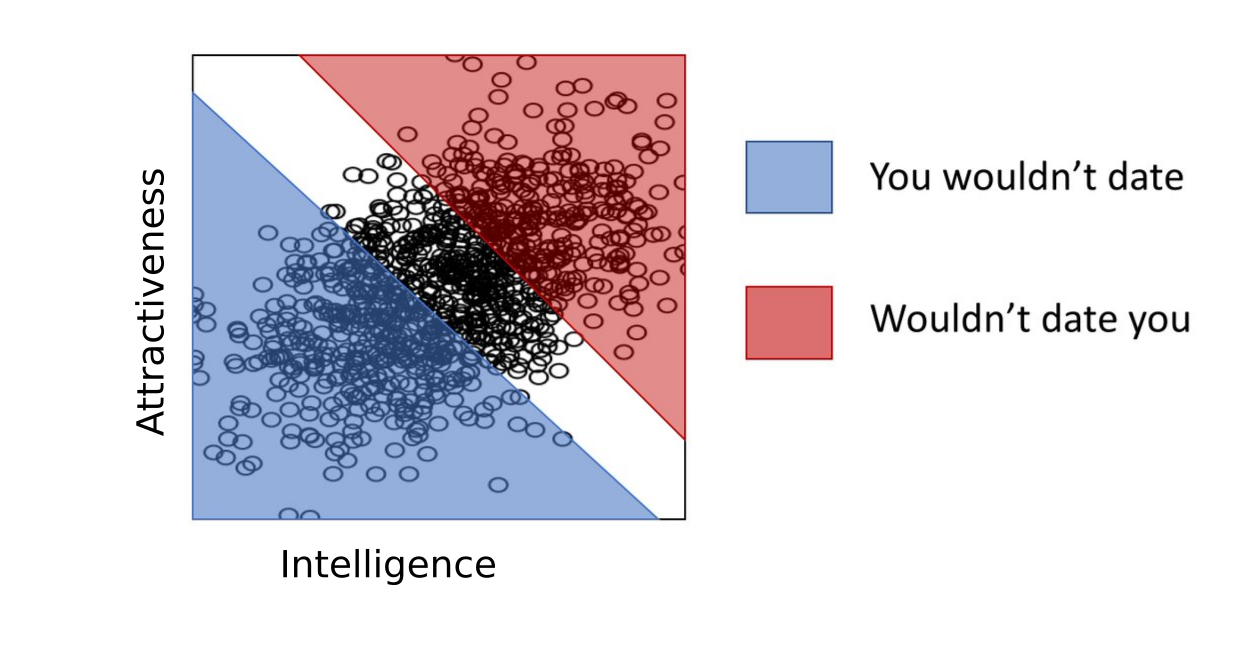
\includegraphics[width=5in]
{berkson/berkson.png}
\caption{
Example
of Berkson's paradox (BP).} 
\label{fig-berkson}
\end{figure}


Fig.\ref{fig-berkson}
presents an example
of BP. The
figure consists of
a scatter plot
with axes $a=$her attractiveness,
$b=$her intelligence, 
for a female  population of 
possible dates for you,
assuming you are a male person.
Let $x\in\{false=0, true=1\}=$
she goes out on a date with you.
For the full population,

\beq
(a,b)\sim P(a,b)=P(a)P(b)
\eeq
whereas for the population
in the white swath,

\beq
(a,b)\sim P(a,b|x)=P(b|a,x)P(a|x)\neq
P(b|x)P(a|x)
\;.
\eeq

As shown by
Fig.\ref{fig-berkson},
 BP is an example of {\bf selection bias}.
Selection bias happens when
a non-representative
subset of the total population
is considered (i.e., selected).


